%
% $RCSfile: record.tex,v $
%
% Copyright (c) 2001-2004. Christian Heller. All rights reserved.
%
% Permission is granted to copy, distribute and/or modify this document
% under the terms of the GNU Free Documentation License, Version 1.1
% or any later version published by the Free Software Foundation;
% with no Invariant Sections, with no Front-Cover Texts and with no Back-Cover
% Texts. A copy of the license is included in the section entitled
% "GNU Free Documentation License".
%
% http://www.cybop.net
% - Cybernetics Oriented Programming -
%
% http://www.resmedicinae.org
% - Information in Medicine -
%
% @author Christian Heller <christian.heller@tuxtax.de>
% @author Jens Bohl <info@jens-bohl.de>
%

\section{Record -- An EHR Module}
\label{record_an_ehr_module_heading}

The practical background for the application of CYBOP is \emph{Res Medicinae}
\cite{resmedicinae}. A modern clinical information system is the aim of all efforts
in this project. In future, it shall serve medical documentation, archiving,
laboratory work etc. \emph{Res Medicinae} is separated into single modules depending
on different tasks.\\
One of these modules is \emph{Record} -- an application for documenting medical
information (figure \ref{record_figure}). In addition to new documentation models,
it also contains a tool for topological documentation.

\begin{figure}[ht]
    \begin{center}
       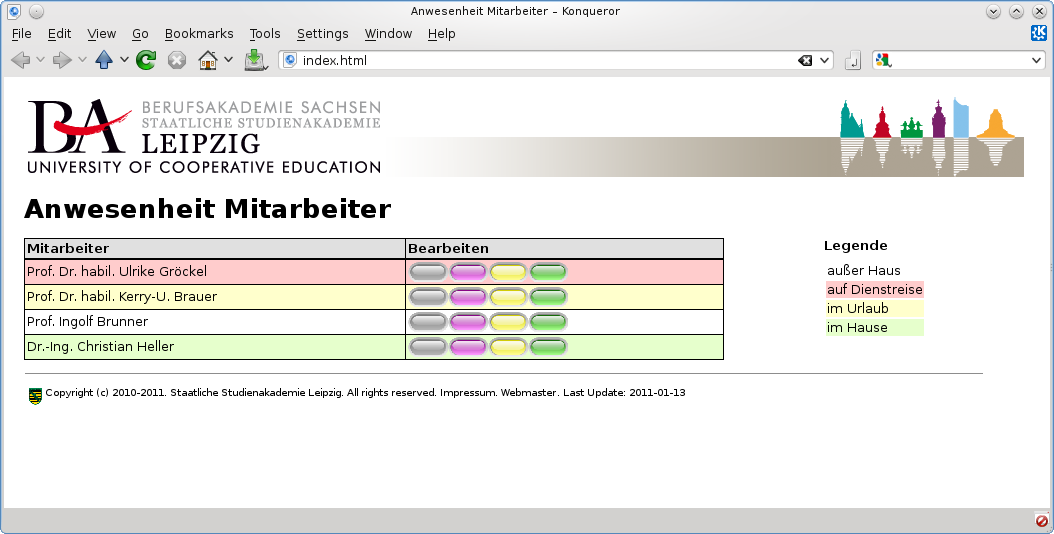
\includegraphics[scale=0.3]{eps/screenshot.eps}
       \caption{Screenshot of Record \cite{urban}}
       \label{record_figure}
    \end{center}
\end{figure}

Starting from an overall view of the human body, it is possible to reach every
organ or region of the body in detail (figure \ref{topology_figure}).

\begin{figure}[ht]
    \begin{center}
       \includegraphics[scale=0.5]{eps/topology.eps}
       \caption{Excerpt from Topological Structure of Human Skeleton}
       \label{topology_figure}
    \end{center}
\end{figure}

